\documentclass[10pt]{ctexart}
\newcounter{myCounter}
\newcommand{\head}[1]{\textbf{#1}}
\newcommand{\keyword}[2][\bfseries]{{#1#2}}
\usepackage{graphicx}
\usepackage[colorlinks,
            linkcolor=red,
            anchorcolor=blue,
            citecolor=green
            ]{hyperref}
\begin{document}


\title{计算实践第二周作业} % This is the title
\author{数33 赵丰 2013012178}
\date{Auguest 26,2016}
\maketitle
\section{Abstract}
分别用显式欧拉法和梯形法给出\fbox{\keyword[\itshape]{Adams-Bashforth}}
求解的初值条件,印证课上讲的两种给初值的方法均是二阶的。
\section{presentation}
\setlength{\parindent}{2em}
  对给定的2步显式的\fbox{\keyword[\itshape]{Adams-Bashforth}} 方法:
  
其第一特征多项式为\(x^2-x=0\),有两个单根\(x=0,1\),故该方法是\keyword{稳定}的。
其局部截断误差为\(T_{n+2}=0.42h^3O(1)\),
其中O(1)为\(y^{(3)}(x_n)\)的量级。 故该方法的收敛阶为2,应选取局部截断误差为$O(h^2)$的单步方法给初值。

若用该方法求解 $$ Y'(t)=-Y(t)+2cos(t),Y(0)=1 $$
该方法的准确解为$Y(t)=sin(t)+cos(t)$用$h=0.1$欧拉法给初值求解后作出其图像如下所示:
\begin{figure}[!ht]
\centering
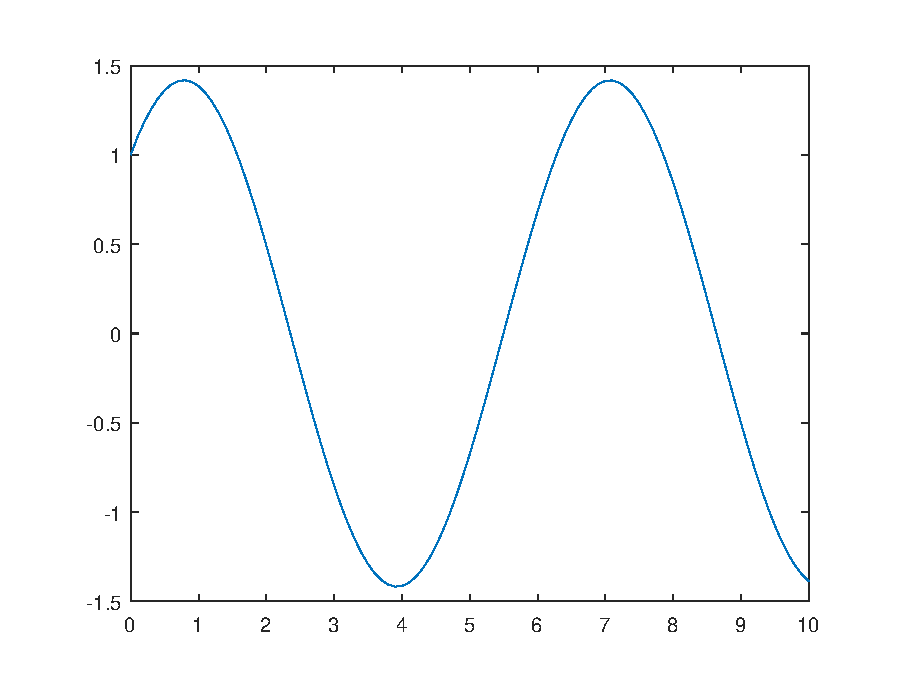
\includegraphics[scale=0.4]{figure1.eps}
\caption{\(sin(x)+cos(x)\)}
\end{figure}

取时间步长分别为$$h=0.1,0.05,0.025,0.0125$$
计算结果如下表所示:\\

\begin{table}[!ht]
\caption{显式欧拉法准备初值 \qquad\qquad\quad 梯形法准备初值}
\begin{tabular}{ccccp{1.5cm}}
\hline
\head{h} & \head{t} & \head{y(t)} & \head{Error} & \head{Relative Error} \\
\hline
0.1 & 1 & 1.38 & 0.003 & 0.002 \\
    & 2 & 0.49 & -0.001 & -0.002 \\
    & 3 & -0.85 & -0.004 & 0.004 \\
    & 4 & -1.41 & -0.003 & 0.002 \\
\hline
\end{tabular}
\begin{tabular}{ccccp{1.5cm}}
\hline
\head{h} & \head{t} & \head{y(t)} & \head{Error} & \head{Relative Error} \\
\hline
0.1 & 1 & 1.38 & 0.0007 & 0.0005 \\
    & 2 & 0.49 & -0.0002 & -0.004 \\
    & 3 & -0.85 & -0.004 & 0.005 \\
    & 4 & -1.41 & -0.003 & 0.002 \\
\hline
\end{tabular}
\end{table}

由上表可以看出t=3之后两种方法的数值误差已经非常接近,更详细的误差表可参见:\href{multiframe.html}{误差表}
由Log-Log图可得到两种方法的收敛阶如下表:\\

\begin{tabular}{ccc}
\hline
\head{h} & \head{显式欧拉法准备初值} & \head{梯形法准备初值}\\
\hline
2  & 1.94 & 1.97\\
3  & 1.99 & 2.00\\
\hline
\end{tabular}

\section{bibliography}

\end{document}